\section{Introduction}
% context
The web is an invaluable source of data and information about virtually any
subject we can think of. Some of this information is made available to the
public in a semi-structured fashion (e.g., shopping items, news, search engine
results, etc.), providing some level of organization that can be exploited and
leveraged: one can use it to detect/find semi-structured content in a document.
But there are other parts of a document, besides the main content, that can have
some sort of organization (template and menus, for instance), this
``non-content'' organized information adds noise to the extraction process,
decreasing precision. How can we distinguish between them? This is the problem
we tackle in this paper.

% motivation
Extracting structured information, by itself, is an important task, but we must
also be able to identify content, distinguish it from noise, so we do not end up
with an unusable, bloated database, full of unimportant information (i.e.,
noise).
According to \cite{Volume05,TPS2013} between 40\%-50\% of a web document refers
to noise (menus, template, ads), this amount is more than enough to completely
compromise extraction precision.
Since structured data can exist in any kind of web document, whether main
content is structured or not, we must be able to identify it correctly
independently from its source, even when there is no structured content, i.e.
we must be able to identify noise in a document whose main content is textual
as well as in a document whose main content is semi-structured.
So, once we have extracted the structured content from a document, how can we
classify it as content or noise? We could not find in literature, nor did we
reach a deterministic and closed form way of doing this, for this reason we
decided to characterize (create hypothesis for the features) content and noise
the best we could and try out machine learning models to approximate a solution.
Our goal is to classify \textbf{structured data}, specifically, as content or
noise, but without restricting ourselves to \textbf{structured content}
documents (i.e., we also want to detect structured noise in textual content
documents). This is a desirable property in order to avoid manual intervention
(selecting only certain types of documents for processing) for the web is
completely heterogeneous in all aspects. But we also evaluated the models in a
controlled setting, when the web pages are known beforehand to have structured
content. This scenario is not unreallistic (e.g., a focused crawler that
retrieves only search result records from e-commerce sites), altought it does
demands more manual intervention.

% related work
Previous attempts at this problem, such as \cite{Densiometric08,Noisy03,
Boilerplate10, vieira2006fast}, were targeted at textual content, their
performance is measured in tasks such as clustering and classification of web
pages, not in terms of records extracted. It is also not clear whether or not
these approaches can be used with structured content, they might remove part of the content,
believing it is noise, without affecting clustering, but this removal would most
likely impair record extraction.
 
% {\textcolor{red}{estás afirmando uma coisa que vais provar? Pelo menos uma
% justificativa dessa tua "crença" deve ser dada, afinal, estás criticando
% trabalhos relacionados e isso não pode ser gratuitamente}}

 Other attempts (\cite{TPS2013,Velloso:2017:ERW:3132847.3132875}), targeted at
structured content, can not be used in an open environment (i.e., one where we
encounter any kind of content: textual, structured  or hybrid), they assume only
structured content will be processed. Although this is not completely
unrealistic it is also not as general, demanding more controlled environments of
execution (i.e., more manual intervention needed).

% {\textcolor{red}{este parágrafo está trazendo a discussão de não
% estruturado, semi-est. e estruturado. Mas isso deve aparecer antes, lá no
% parágrafo da motivação... até aqui, não está claro o que tu vais
% consideradar... o título fala em "detectar conteúdo estruturado", mas a tua
% fonte vai ser como? não estruturado, semi-est. e estruturado? não está
% claro}%}

% {\textcolor{red}{os desafios de resolver o problema não vão ser
% discutidos?"How can we distinguish between noise and useful content?" Alguém
% pode achar que é fácil :-) convença-os de que não é :-)}%}

% {\textcolor{red}{eu acho que é necessário uma motivação para o uso destas
% técnicas de ML... da mesma forma que aquele revisor (do email que te mandei)
% comentou, alguém pode dizer que "estão simplesmente testando um monte de
% técnica de ML em cima de um problema"... "qual é o tcham do negócio?"}%}

% proposed approach
%\textcolor{red}{ eu acho que aqui neste par�grafo deveria deixar mais
% expl�cito, tecnicamente, do que se trata o trabalho publicado no CIKM. N�o precisa
%explicar, mas mostrar a intu���o do uso de processamento de sinais; afinal,
%todas as tuas features foram extra�das considerando a ideia que est� l�... e
%isso n�o est� dito em lugar algum }

In this paper, we analyze several possible supervised machine learning models
for structured content detection. Our investigation considered eight machine
learning techniques (Logistic Regression, Gaussian Naive Bayes, k Nearest
Neighbours, Support Vector Machine, Extra Trees, Gradient Boosting, Voting and
Stacking Ensembles) and all possible combinations of features within each
approach to find the one that suited best in each case. For the extraction phase
we choose the method proposed in \cite{Velloso:2017:ERW:3132847.3132875} because
of the good quality of the results, its feasibility in a production environment
(it is unsupervised and computationally efficient compared to other
state-of-the-art approaches) and also because its source code is freely
available for download, allowing reproducibility of results.
This extraction method uses a signal processing approach to detect repetitive
structural patterns in the document by means of stability and spectral analysis.
The web page is converted to a sequence (or signal) representation, prior to
extraction, and it is from this sequence that we derive the features used in our
work.
% {\textcolor{red}{parecem justificativas meio esquisitas para usar um trabalho
% que foi feito pelos autores, né? :-) "... its source code is freely
% available". Acho que dá para ser mais direto e colocar apenas que as
% justificativas técnicas e fim de papo}}
The features proposed here are produced during the extraction phase, we just
normalize their values, adding no overhead to the pipeline (once we have the
model trained). We have attained 94\% F-Score in a dataset consisting of 266
different HTML documents from various domains with structured content and 90\%
F-Score in a dataset with 327 different HTML documents, some with unstructured
content (same 266 structured documents, plus 61 unstructured documents mostly
from blogs, news, etc.).
The novelty presented here lies in the nature of the features. We are using an
alternative representation for the web documents, to the best of our knowledge
this representation was first introduced in \cite{TPC09}, and until now we have
not found any content/noise detection proposal using features derived from this
representation. Our investigation showed these features can be used to solve
this problem effectively and efficiently.
% {\textcolor{red}{DOM tree?? como assim, de onde saiu? Não fale em DOM tree na
% introdução, se estás em um nível de abstração maior... aqui, por
% enquanto, é tudo HTML documents}}

% organization
The rest of this paper is organized as follows: in Section \ref{sec:related} we
present a brief review of related works; in Section \ref{sec:prelim} we
reproduce some concepts needed for the understanding of our work; in Section
\ref{sec:content} we describe and illustrate each feature used in solving the
problem of content detection; in Section \ref{sec:exp} we detail and discuss the
experiments conducted; in Section \ref{sec:results} we analyze the results
achieved and; in Section \ref{sec:con} we present our conclusions.

\section{Related Work}\label{sec:related}

In our research we have encounter quite a few proposals for web page noise
removal, dating as far back as 1999 \cite{kushmerick1999learning}. Most early
works focused in textual content, where main applications were web page
clustering and classification.

In \cite{Densiometric08,Boilerplate10, vieira2006fast, BlockImp07} the main
content of a web page is assumed to be textual, they might be a fit for a web
page with structured content, but that is unlikely and we have no results
published using these techniques for this purpose, as far as we know.

On the other hand, if we assume content is structured
(\cite{TPS2013,Velloso:2017:ERW:3132847.3132875}) we loose generality and became
confined in this setting. An approach biased toward structured content works
great in a controlled environment but can not perform well in an open
environment where we may encounter textual and hybrid content as well, precision
would drop drastically. There is a cost (usually manual intervention and usually
high) associated with maintaining such a well controlled environment.

% colocar mais referencias aqui
We also found many proposals that do not assume content to be structured or
textual (\cite{Noisy03,Jointop07,SiteOriented11,Entropy09}), but each has some
limitation we intend to overcome in our work. In
(\cite{Jointop07,SiteOriented11,Noisy03}) several samples from the same template
are necessary to train the model, and it only works for that particular
template; and in (\cite{Entropy09}) predefined knowledge bases are required.

Much has changed, since this area of research has started, new applications have
arisen, web development culture has changed, among other things. Due to the
web's ever changing nature, any proposal based on too specific assumptions
(content form, predefined knowledge, template specific, static heuristics rules,
etc.) is deemed to rapidly become outdated.

\section{Preliminaries}\label{sec:prelim}
In this section we outline some concepts needed for the understand of our
proposal.

Since we are proposing a way of identifying structured content and noise, we
need to build our work on top of an extraction technique. We chose the approach
reported in \cite{Velloso:2017:ERW:3132847.3132875} for two reasons: i) the
results reported are equivalent to other state-of-the-art approaches and; ii)
the computational complexity is lower, specially when compared to
rendering-based approaches. This extraction technique uses an alternative
representation for the web documents, a \textbf{tag path sequence} (or TPS), and
here we detail this representation. The understanding of this alternate
representation is needed because the features we use to classify content and
noise are derived from it. For a more thorough explanation we refer the reader
to the work in \cite{Velloso:2017:ERW:3132847.3132875}.

\begin{definition}\textbf{(Tag Path)} is a string describing the path from the
root node of the DOM tree to every other node in the tree. For example:
``\texttt{html/body/table/tr/td/\#text}''.
\end{definition}

\begin{definition}\textbf{(Tag Path Code -- TPCode)}\label{def:tpc} is a numeric
ascending code assigned to every different tag path string encountered in the
tree, in order of appearance. If a given path has occurred in the past, it is
assigned the same code as before. The paths are built in depth first order.
Figure \ref{fig:tree2seq} shows an example of this definition. Here we refer to
TPCode as ``symbol'' and a set of TPCodes as ``alphabet''.
\end{definition}

\begin{definition}\textbf{(Tag Path Sequence -- TPS)} is a sequence of TPCodes
in the same order as they were built from the DOM tree. Figure
\ref{fig:tree2seq} shows the resulting TPS for an HTML snippet as  well as the
set of TPCode used for that the sequence. In this paper we also refer to TPS as
simply ``sequence''.
\end{definition}

The translation process from DOM tree representation to tag path sequence is
depicted in Figure \ref{fig:tree2seq}. The HTML code is converted to a DOM tree
in Step 1; the DOM tree is converted to a sequence of tag paths in Step 2 and;
in Step 3 the TPS is built by assigning TPCodes to each tag path. 

\begin{figure}[h]
  \centering
     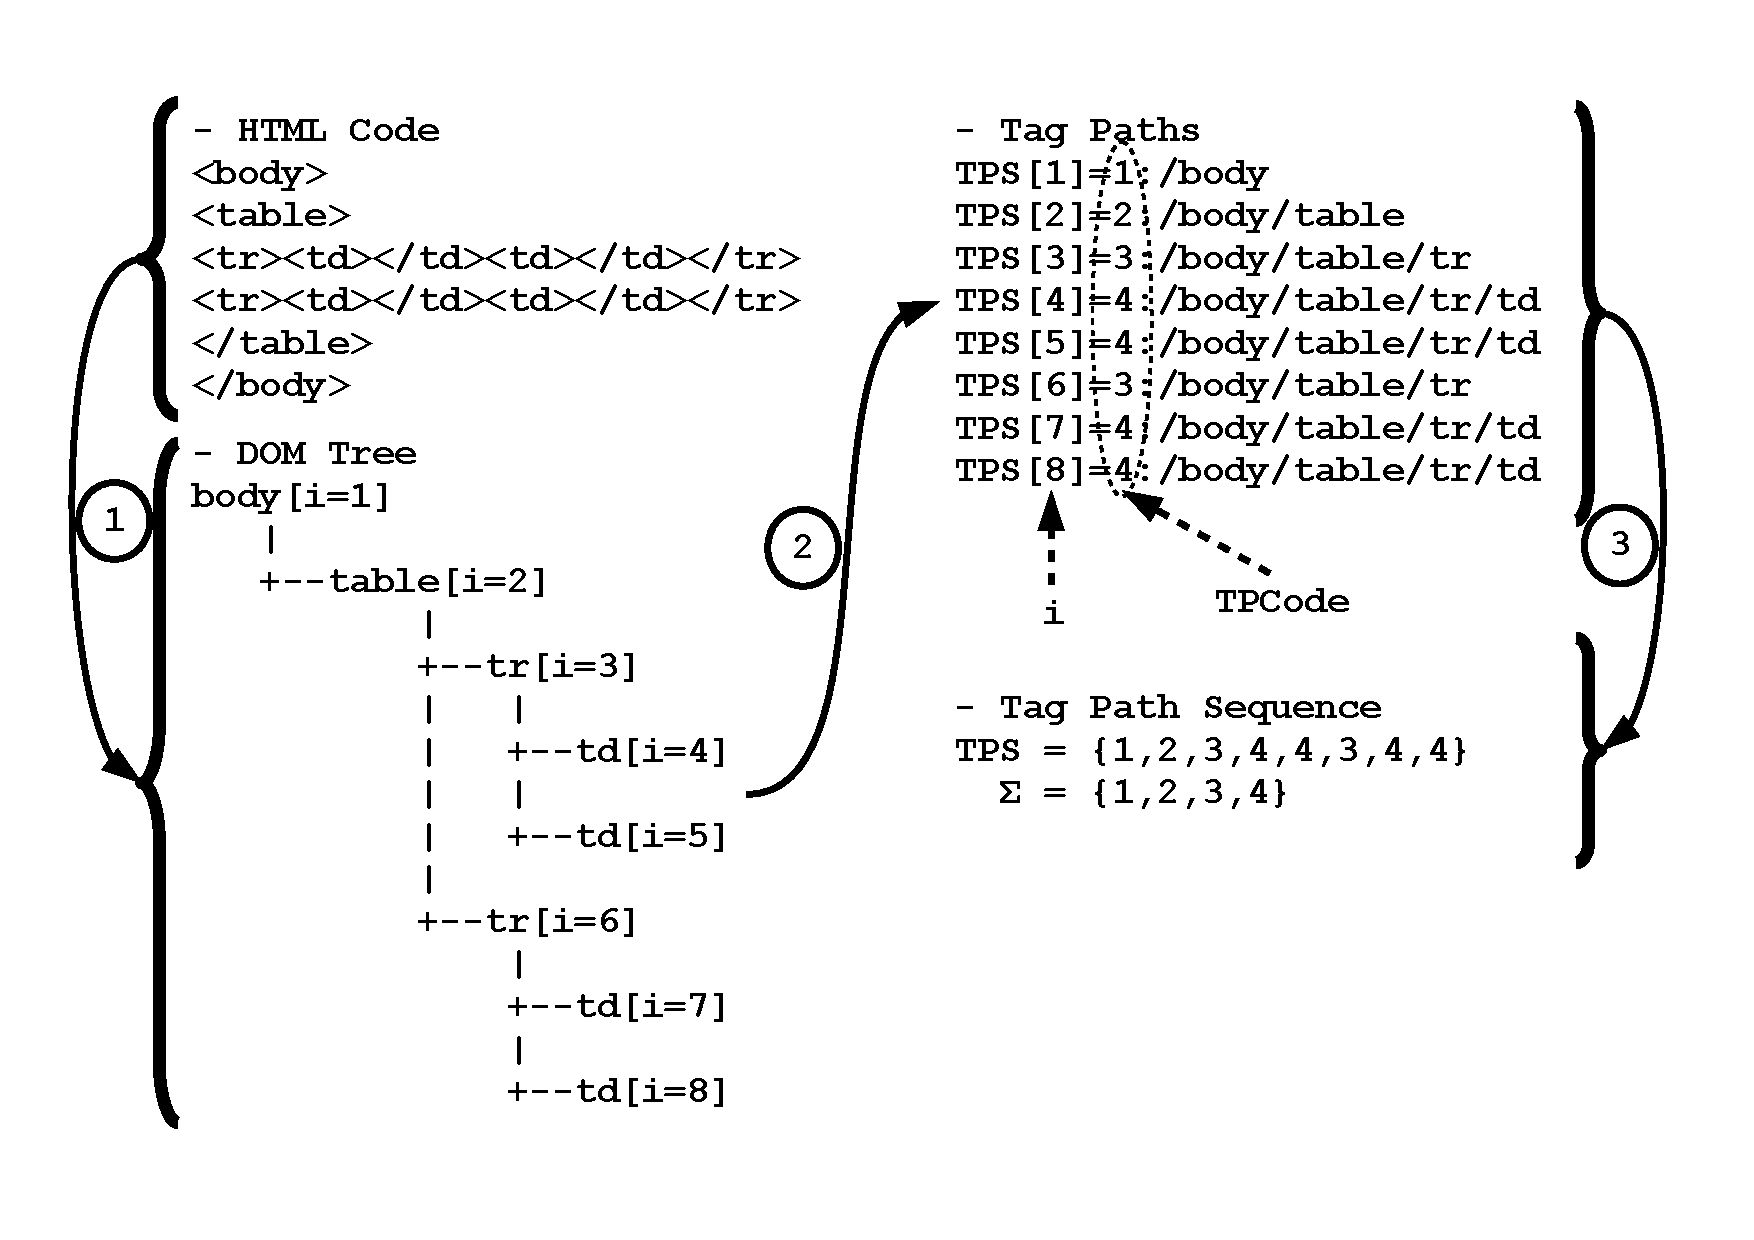
\includegraphics[trim={1.0cm 2.0cm 1.5cm 1.0cm}, clip, 
     width=1.0\columnwidth]{img/tree2seq.pdf}
  \caption{Conversion of HTML snippet to a tag path sequence.}
  \label{fig:tree2seq}
\end{figure}

\section{Content Detection}\label{sec:content}
\textcolor{red}{ n�o vais explicar a intui��o de como as features s�o extra�das?
Afinal, teu documento � representado como um sinal e todas as features s�o
extra�das com base em valores detectados neste sinal; n�o � isso? Deve ficar
claro isso aqui. Outra coisa, tem bastante espa�o sobrando... acho que poderias
fazer uma figura similar �quela que tem no CIKM com a p�gina original e o que
foi gerado dela (n�o a mesma, por favor!)}

In order to distinguish which structured regions are content and which are noise
we consider six region features, such as: size, center position, horizontal
position, vertical position, range and record proportion (record count vs
record size).

These features were chosen because we believe (that is our hypothesis) they
characterize the problem well and thus, can be helpful in solving the problem.
As an extra, they can also be easily acquired from the extraction technique we
are relying on.

We will discuss each feature (size, positions, range and record proportion) in
Subsections \ref{ss:size}, \ref{ss:pos}, \ref{ss:range} and \ref{ss:rec}
respectively.

\textcolor{red}{as Figuras 2, 3 e 4 n�o est�o claras... quero dizer, est�s explicando que s�o um exemplo de documento com cada feature, mas n�o explica o que significam as coordenadas (x e y) nem o que s�o as linhas plotadas. Antes de entrar nos exemplos, tens que dizer que as figuras representam tal coisa, explicando as coordenadas e as linhas plotadas.}

\subsection{Size Feature}\label{ss:size}
The region size feature is a real number, between 0 and 1, that represents the
size of the region relative to the entire document, i.e., the percentage of the
document occupied by the region.

The idea behind this feature is that if a web document was designed with the
purpose of depicting a specific content, then this content (the reason the
document was created in the first place) should occupy a considerable portion of
the document. That is, our hypothesis is that the likelihood of a region being
content (and not noise) is directly proportional to its size.

\begin{figure}[h]
  \centering
     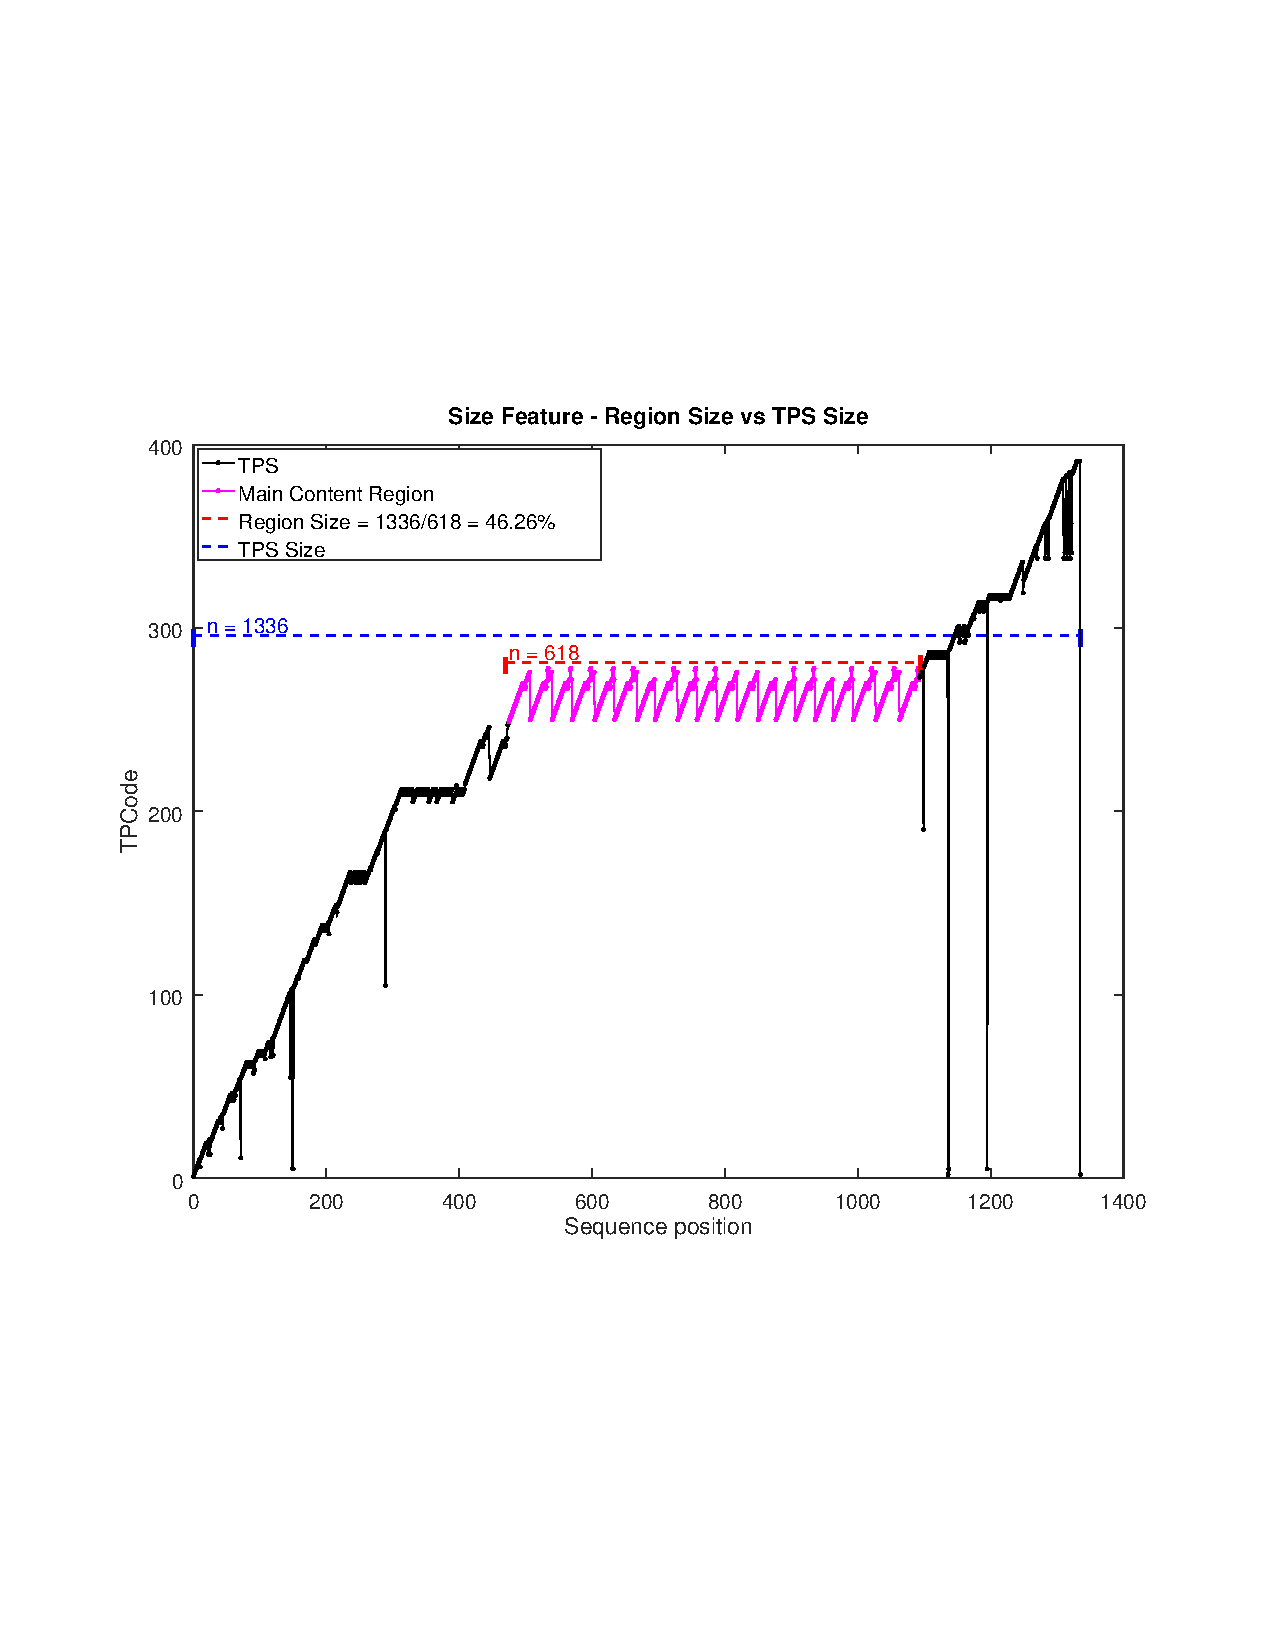
\includegraphics[trim={2.5cm 7.4cm 2.2cm 7.4cm}, clip,  width=\columnwidth]{img/size.pdf}
  \caption{Size feature example.}
  \label{fig:size}
\end{figure}

Figure \ref{fig:size} shows an example where the entire document sequence has
size equal to 1,336 and the main content region subsequence has size 618. The
size feature in this case, using Equation \ref{eq:size}, is equal to
$\frac{618}{1,336} = 46.25\%$.

\begin{equation}\label{eq:size}
    sizeFeat = \frac{regionSize}{sequenceSize}
\end{equation}

\subsection{Position Features}\label{ss:pos}
The region position feature is actually comprised of three position features:
center, horizontal and vertical positions. All three are real numbers between 0
and 1. The \textbf{center position} represents the distance from the center of
the region to the center of the document; the \textbf{horizontal position} is
the distance from the center of the region to the end of the document and; the
\textbf{vertical position} is the distance from the vertical center of the
region to the maximum value of the sequence.

With respect to the center position, the maximum possible distance is equal to
half sequence size (e.g, when a region has size one and sits at the start/end of
the document). The value of this feature is a percentage representing how close
a region is from the center of the document (i.e., it is the distance
complement). The rationale of our hypothesis for this feature is similar to the
size feature (Subsection \ref{ss:size}): the closer a region is to the center of the
document, the higher the probability it refers to real content.

\begin{figure}[h]
  \centering
     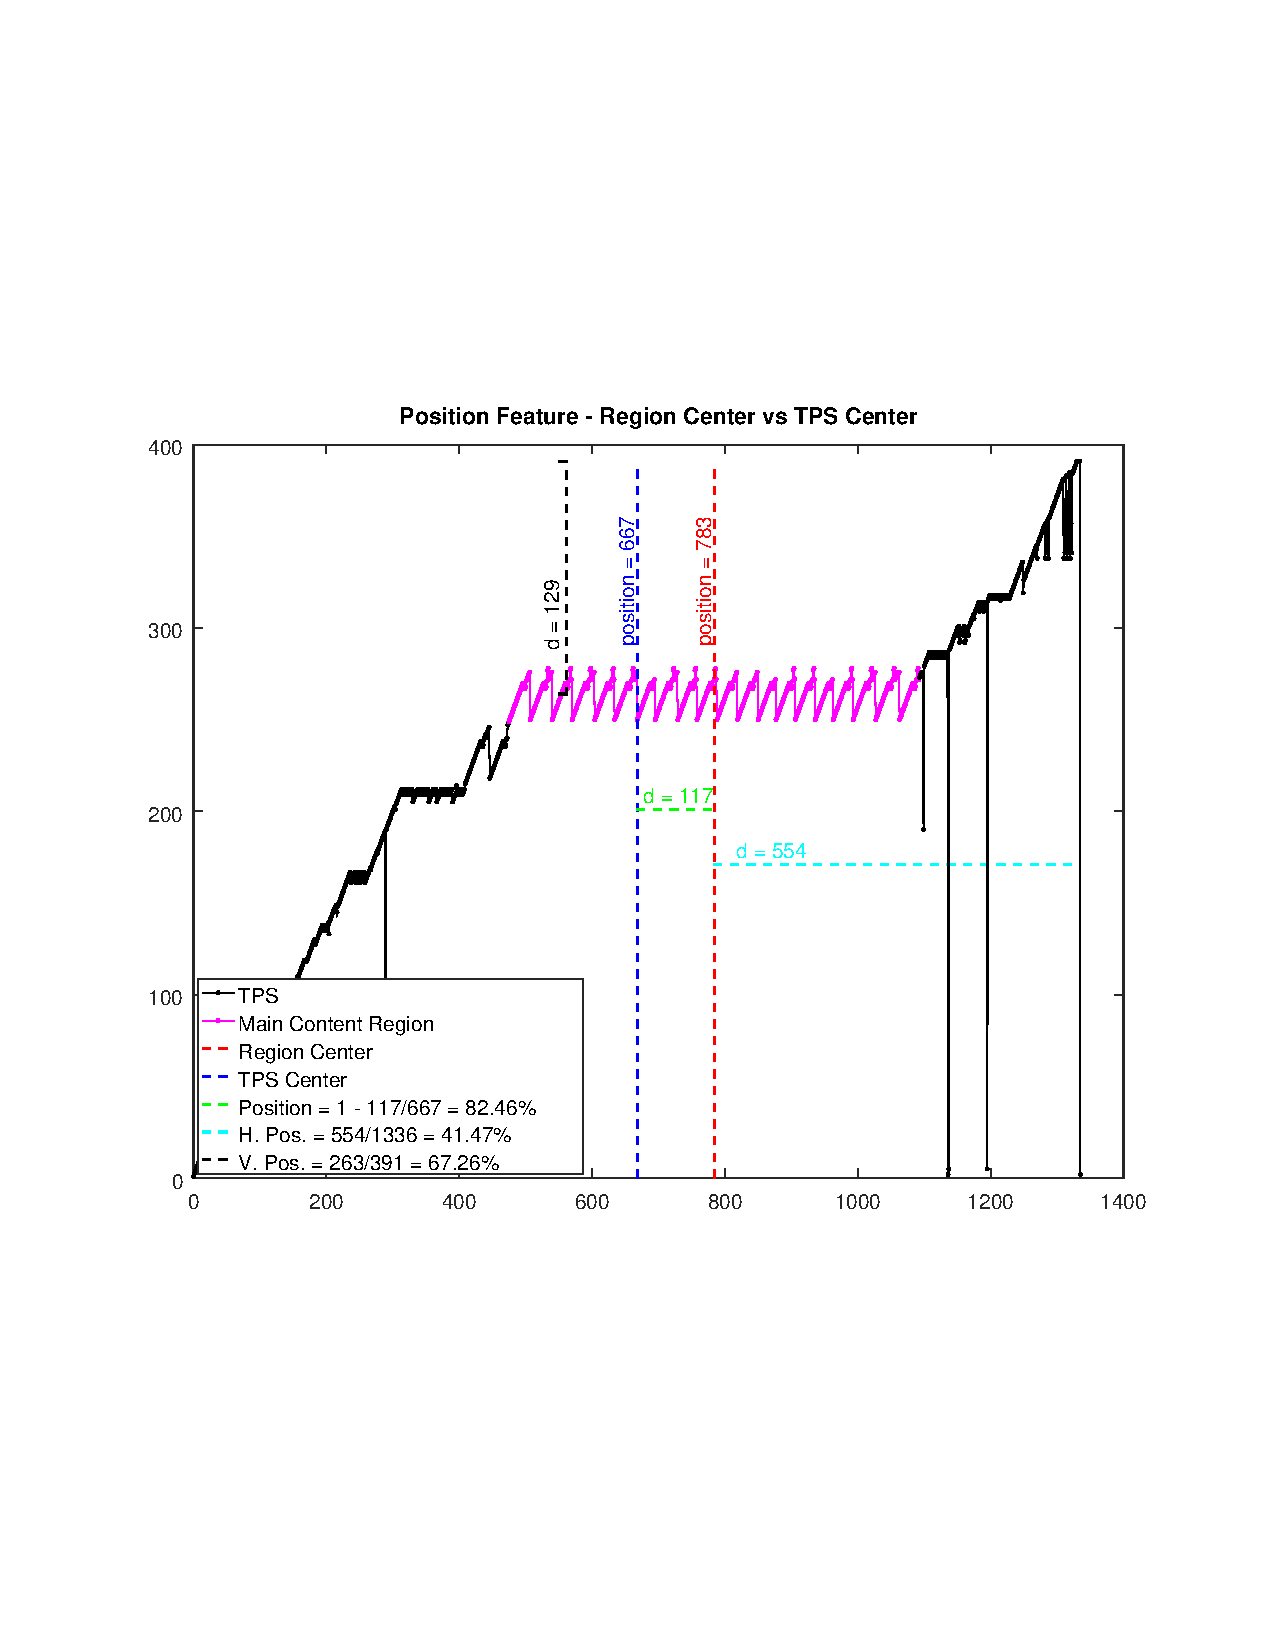
\includegraphics[trim={2.5cm 7.4cm 2.2cm 7.4cm}, clip,  width=\columnwidth]{img/position.pdf}
  \caption{Position feature example.}
  \label{fig:position}
\end{figure}

Figure \ref{fig:position} shows an example where the document center is at
position 667 (this is the maximum distance allowed) and main content region
subsequence center is at position 783, at a distance of 117 from document
center. The value of this feature, using Equation \ref{eq:cposition}, is equal
to $1- \frac{117}{667} = 82.46\%$

\begin{equation}\label{eq:cposition}
    centerPositionFeat = 1 - \frac{|regionCenter - sequenceCenter|}{sequenceCenter}
\end{equation}

With respect to the vertical and horizontal position, we believe they are needed
to provide a better indication of a region's position, \textbf{specially} when a
document has no structured content (only structured noise), in this situation a
noise region will be closer to the center of the sequence and further away from
its extremes. If we were concerned only about documents with structured content,
these two features would, probably, be of little value to us.

Figure \ref{fig:position} shows how the horizontal and vertical positions are
calculated. The horizontal position is the distance from the center of the
region to the end of the sequence. Using Equation \ref{eq:vposition}, the value
of the horizontal position, in this example, is equal to $\frac{554}{1,336} =
41.47\%$.

\begin{equation}\label{eq:hposition}
    horizontalPositionFeat = \frac{sequenceSize - regionCenter}{sequenceSize}
\end{equation}

The vertical position is the distance from the vertical
center of the region (i.e., its average value) to the vertical end of the
sequence (i.e., its maximum value). Using Equation \ref{eq:vposition}, the value
of the vertical position, in this example, is equal to $\frac{263}{391} =
67.26\%$.

\begin{equation}\label{eq:vposition}
    verticalPositionFeat = \frac{avg(region)}{max(sequence)}
\end{equation}

Throughout this paper we will refer to these features as ``center'',
``horizontal'' and ``vertical'' features.

\subsection{Range Feature}\label{ss:range}
The range feature is a real number, between 0 and 1, that represents the
percentage of the region range relative to the entire sequence. It is analogous
to the Size Feature (Subsection \ref{ss:size}) only it is vertical instead of
horizontal. The region range is simply the maximum value found in the sequence
(or subsequence) minus the minimum value and the sequence range is equivalent
to its maximum value.

\begin{figure}[h]
  \centering
     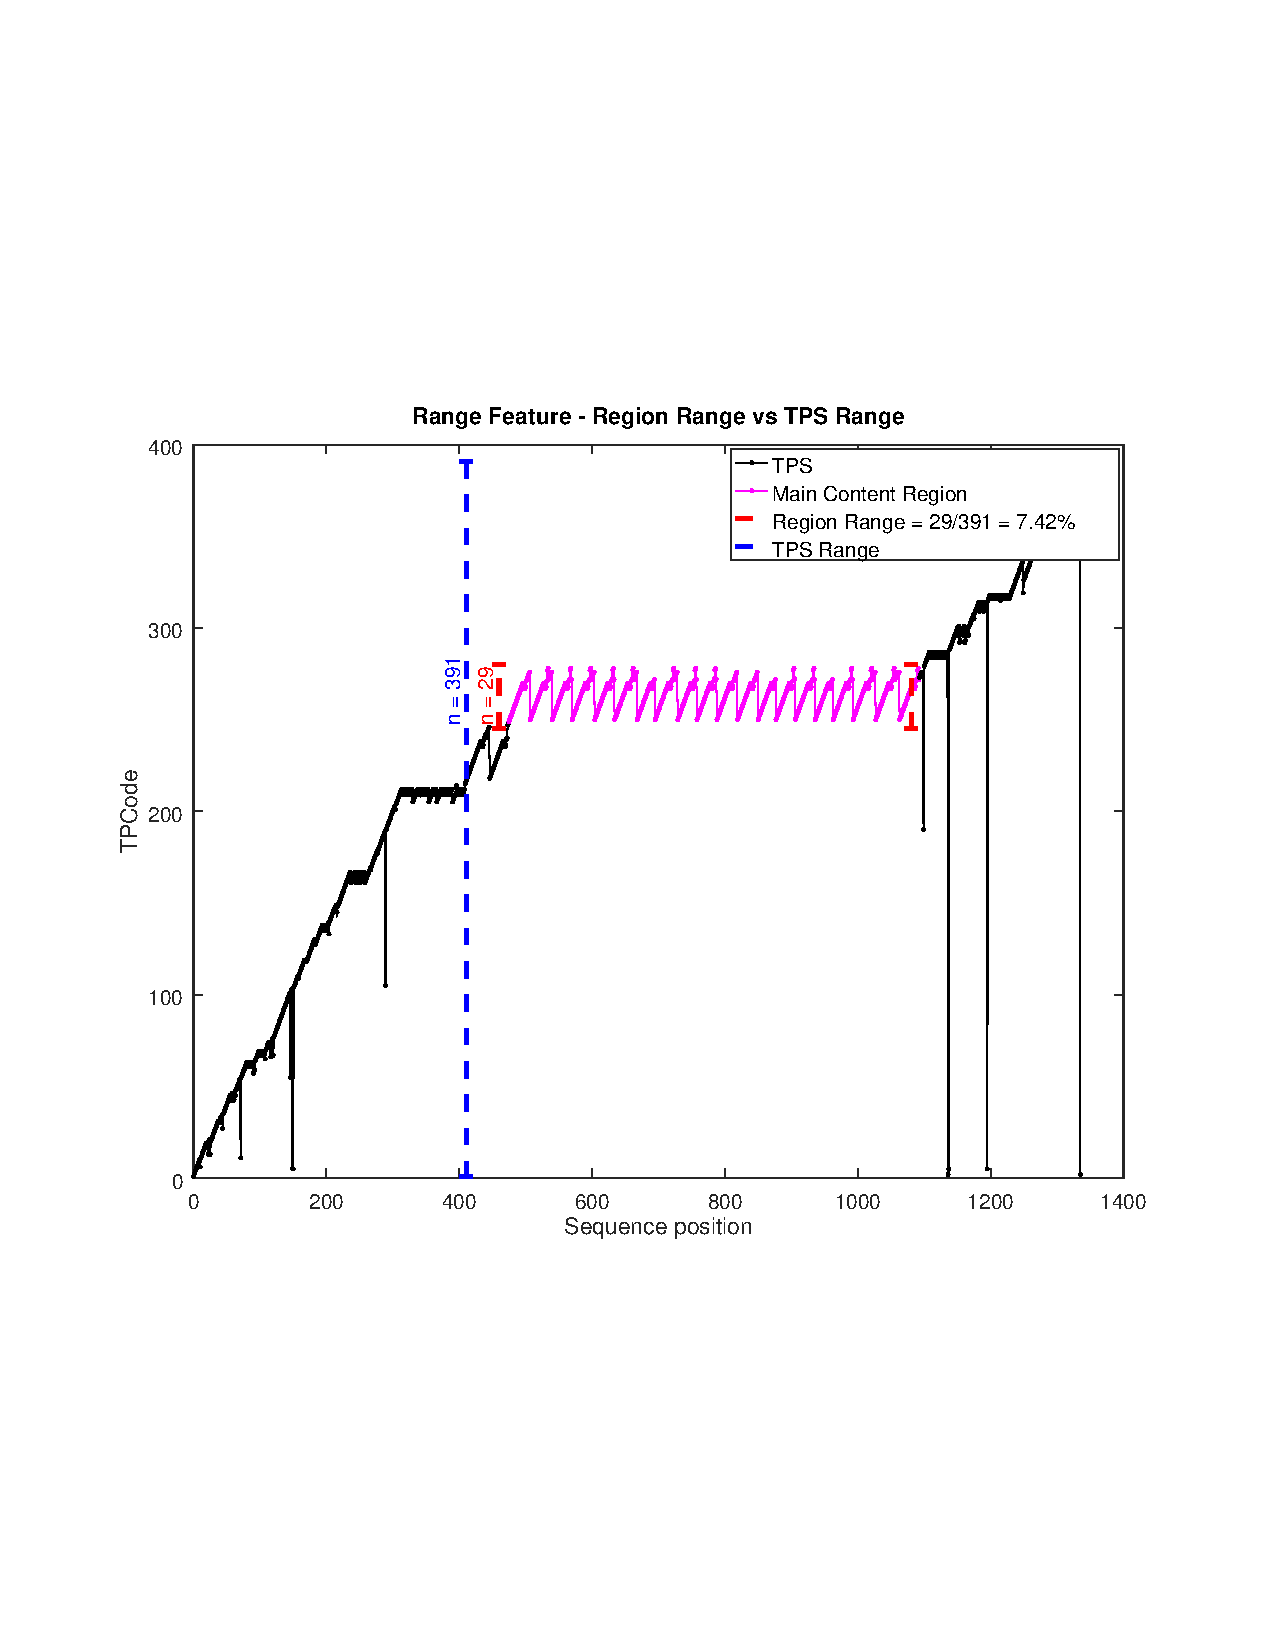
\includegraphics[trim={2.5cm 7.4cm 2.2cm 7.4cm}, clip,  width=\columnwidth]{img/range.pdf}
  \caption{Range feature example.}
  \label{fig:range}
\end{figure}

Figure \ref{fig:range} shows an example where region range is equal to 29 and
document range is equal to 391. The value of this feature, using Equation
\ref{eq:range}, is equal to $\frac{283-254}{391}=\frac{29}{391}=7.42\%$ of
document range.

\begin{equation}\label{eq:range}
    rangeFeat = \frac{regionRange}{max(sequence)}
\end{equation}

\subsection{Record Feature}\label{ss:rec}
We use the ratio between the number of records and their average size as a
feature to indicate if a region is content or noise. We hypothesize that the
lack of proportion\footnote{i.e., a lot of small records or few large records}
between this two measures (record count and record size) indicates noise and,
conversely, the closer they are from one another the more likely the region is
content. We calculate this value as shown in Equation \ref{eq:recsize}.

\begin{equation}\label{eq:recsize}
recRatioFeat = \frac{min(numRecs, recCount)}{max(numRecs, recCount)}
\end{equation}

The value of this feature is also a real number between 0 and 1, since the
denominator in Equation \ref{eq:recsize} is always greater or equal to the
numerator.

This two measures are obtained as documented in
\cite{Velloso:2017:ERW:3132847.3132875}, using the region's power spectrum
density (PSD).
Figure \ref{fig:fft} shows the PSD of the main content region
and its detected record count and average record size. In this example the
number of records detected is 20 and their average size is 31, so the value of
the feature, using Equation \ref{eq:recsize}, is equal do $\frac{20}{31}=64.51\%$

\begin{figure}[h]
  \centering
     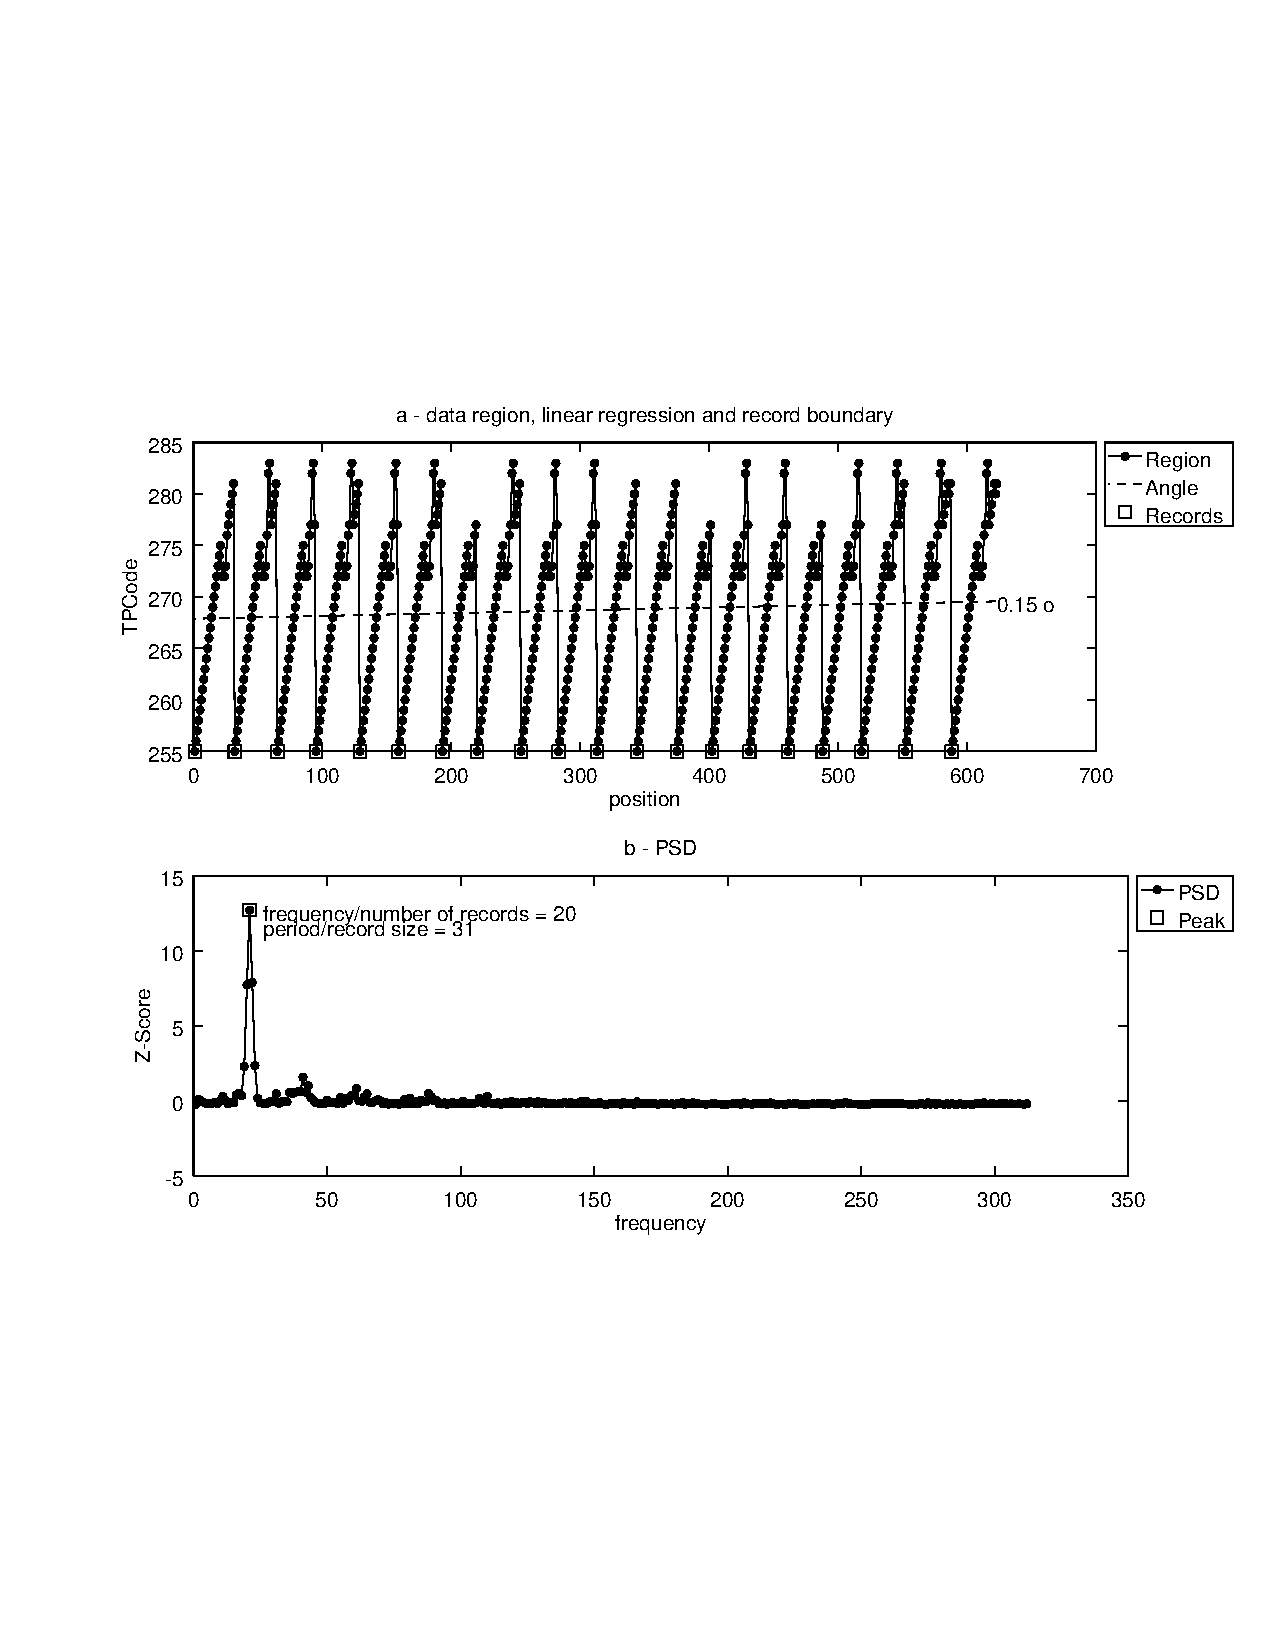
\includegraphics[trim={2.0cm 7.4cm 0.7cm 7.4cm}, clip,  width=\columnwidth]{img/fftreg.pdf}
  \caption{Record count \& size feature example.}
  \label{fig:fft}
\end{figure}

\textcolor{red}{a Figura 5 est� bem mal explicada... :( sei que est�s referenciando o artigo do CIKM, mas pelo menos explique o que significa. A figura em si tem duas imagens, e quando falas por exemplo que o n�mero de registro � 20, o leitor fica confuso se isso deve ser visto na primeira imagem ou na segunda. Coloque (a) e (b) em cada uma delas e explique melhor o que elas representam. Al�m disso, claro ela foi gerada a partir de que outra imagem? (na verdade, a primeira imagem � um "corte" de uma regi�o e isso n�o est� claro}

Throughout this paper we will refer to this feature as ``record'' feature.

%\subsection{Angular Coefficient}\label{ss:ang}
%The angular coefficient is used in \cite{Velloso:2017:ERW:3132847.3132875}
%during extraction to detect if a region is structured or not. A low coefficient
%is an indication of structure. We have not constructed an hypothesis around
% this features, we employ it here to investigate if it is also helpful in
%discriminating content from noise.

%Figure \ref{fig:fft} shows the main content region's angular coefficient (0.15
%degrees). We calculate the feature value using Equation \ref{eq:angle}. The
%value of this feature is a real number, between 0 and 1 and it is inversely
%proportional to the region angle since a low angle is an indication of
% structure and the value is relative to the maximum possible angle, which is 45 degrees
%(maximum angle is achieve when there is no structure whatsoever).

%\begin{equation}\label{eq:angle}
%    angleFeat = 1 - \frac{|angularCoeff|}{\frac{\pi}{4}}
%\end{equation}

%Figure \ref{fig:fft} shows an example where the angle is 0.15 degrees. This
%angle corresponds, approximately, to an angular coefficient of 0.0027047, using
%Equation \ref{eq:angle} the feature value is equal to
%$1-\frac{0.0027047}{\frac{\pi}{4}}=99,65\%$

\section{Experiments}\label{sec:exp}

% {\textcolor{red}{em vez de "to achieve the goal of content detection" eu seria
% bem direta e faria um parágrafo que apresente, em uma frase, o(s) objetivo(s)
% dos experimentos (cujos resultados serão apresentados pelas metricas de
% avaliacao com numero plotados nos gráficos)}%}

In this section we detail the experiments we conducted using supervised machine
learning techniques with the features from Section \ref{sec:content}. We also
characterize the dataset used in the experiments, its statistical propoerties,
features correlation, etc. The objectives of this experiments are to determine
the parameters and the subset of features which are important in this
classification problem and measure the classification performance in terms of
precision, recall, accuracy and f-score.

We have considered, in our study, the following machine learning techniques:
gaussian naive Bayes (GNB), logistic regression (LR), k Nearest Neighbours
(kNN), Gradient Boosting (GB), Extra-trees (EXT), Support Vector Machine (SVM),
Voting Ensemble (VOT) and Stacking Ensemble (STCK). The voting and stacking
ensembles are heterogeneous ensembles and are built from combinations of all the
other models (GNB, LR, kNN, SVM, GB and EXT). These experiments were conducted
using scikit-learn\cite{scikit-learn} framework. For the gradient boosting we
used XGBoost\cite{Chen:2016:XST:2939672.2939785} and for the ensembles we used
MLxtend's\cite{raschkas_2018_mlxtend} implementation.

We have conducted experiments to determine the best combination of parameters
and features, within each approach, for solving the problem of distinguishing
noise from content. To do so we ran a grid search for each algorithm with all
feature combinations since the number of possible combinations, for six
features, is not prohibitive (only 63 in total).
After that we have used grid search, again, to select the best parameters for
each algorithm. The feature set for each algorithm is documented in Table
\ref{tab:featsel} and the parameters in Table \ref{tab:params} (more details
on that in Section \ref{sec:results}).

For these experiments we have used a dataset consisting of 266 HTML documents
with structured content from various domains (news, banking, hotels, car rental,
tickets, electronics), plus 61 documents \textbf{without} structured content,
totalizing 327 documents. The documents without structured content were added to
the dataset to investigate the behaviour of the classifiers in the presence of
this type of input.
We use only one page per site to avoid introducing bias towards specific sites
and/or templates\footnote{this is possible because the extraction approach used
also works with a single page input}. These documents were processed using the
technique proposed in \cite{Velloso:2017:ERW:3132847.3132875}, resulting in a
total of 533 regions that were manually labeled as content or noise (menus, ads,
template, etc). This is the input dataset used for training and cross-validation
and it is summarized in Table \ref{tab:dataset}. Figure \ref{fig:dataset} shows
a scatter plot of each feature, separately, with respect to the target class
(content vs noise), it gives a rough idea of how content and noise are
intertwined. 

Table \ref{tab:stat} shows mean, coefficient of variation (CV), skewness and
kurtosis for all features with respect to the target class. Table
\ref{tab:featcorr} shows the correlation between all features. We see that
``size'' vs ``position'', ``size'' vs ``range'' and ``position'' vs ``range''
have a stronger correlation compared to others, this fact reflected in feature
selection for some models.
These same three features, according to Table \ref{tab:importance}, are also
the most important ones. The ranking of features, with both criterias (ANOVA and
$\chi^2$) yielded the same result.

% \textcolor{red}{as legendas das figuras estao iguais... além disso, eu
% colocaria a legenda de noise e content mais visivel (está escondida, eu
% demorei para achar ...:) ) }
 
\begin{table}[h]
\centering
\caption{Input dataset summary.}
\label{tab:dataset}
\begin{tabular}{ | l | l | r |}
\hline
\# Content Regions & 254 & 47.65\% \\
\# Noise Regions & 279 & 52.35\% \\
\hline
Total & 533 & 100\% \\
\hline
\# Structured documents & 266 & 81.35\% \\
\# Unstructured documents & 61 & 18.65\% \\
\hline
Total & 327 & 100\% \\
\hline
\end{tabular}
\end{table}

\begin{table}[h]
\centering
\caption{Relative Feature Importance (feature vs class).}
\label{tab:importance}
\begin{tabular}{| l | l | l |}
\hline
feature & $\chi^2$ & ANOVA \\
\hline
Size       & 51.6426225  & 487.50116318 \\
Center     & 25.8025951  & 260.93679423 \\
Range      & 23.1719961  & 232.44608713 \\
Record     & 4.71168623  & 26.59572956 \\
Vertical   & 1.16942710  & 12.38250104 \\
Horizontal & 0.433793117 & 3.63505065 \\
\hline
\end{tabular}
\end{table}
         
\begin{table}[h]
\centering
\caption{Correlation between all features.}
\label{tab:featcorr}
\begin{tabular}{ | l | l | l | l | l | l |}
\hline
& Size & Record & Range & Horizontal & Vertical \\ \hline
\multicolumn{6}{|l|}{Content \& Noise} \\
\hline
Center & \textbf{0.63} & 0.08 & 0.45 & -0.11 & 0.01 \\
Size & & 0.08 & \textbf{0.68} & -0.02 & 0.11 \\
Record & & & 0.08 & 0.04 & 0.03 \\
Range & & & & -0.01 & 0.08 \\
Horizontal & & & & & \textbf{0.85} \\
\hline
\multicolumn{6}{|l|}{Content} \\
\hline
Center & 0.58 & -0.11 & 0.21 & -0.37 & -0.07 \\
Size & & -0.10 & 0.53 & -0.12 & 0.12 \\
Record & & & -0.04 & 0.04 & -0.04 \\
Range & & & & -0.03 & 0.08 \\
Horizontal & & & & & 0.65 \\
\hline
\multicolumn{6}{|l|}{Noise} \\
\hline
Center & 0.25 & -0.01 & 0.22 & -0.15 & -0.11 \\
Size & & -0.12 & 0.39 & -0.15 & -0.11 \\
Record & & & -0.08 & 0.01 & 0.01 \\
Range & & & & -0.13 & -0.09 \\
Horizontal & & & & & 0.89 \\
\hline
\end{tabular}
\end{table}

\begin{table}[h]
\centering
\caption{Feature statistics.}
\label{tab:stat}
\begin{tabular}{ | l | l | l | l | l |}
\hline
Feature & Mean & CV & Skewness & Kurtosis \\
\hline
\multicolumn{5}{|l|}{Content \& Noise} \\
\hline
Size & 0.27 & 0.87 & 0.92 & 2.90 \\
Center & 0.57 & 0.51 & -0.18 & 1.71 \\
Range & 0.11 & 1.12 & 1.98 & 7.46 \\
Record & 0.40 & 0.68 & 0.52 & 2.15 \\
Vertical & 0.59 & 0.40 & -0.49 & 2.42 \\
Horizontal & 0.55 & 0.47 & -0.26 & 2.14 \\
\hline
\multicolumn{5}{|l|}{Content} \\
\hline
Size & 0.44 & 0.49 & 0.28 & 2.47 \\
Center & 0.74 & 0.27 & -0.81 & 2.95 \\
Range & 0.19 & 0.74 & 1.49 & 5.51 \\
Record & 0.46 & 0.61 & 0.22 & 1.89 \\
Vertical & 0.63 & 0.24 & -0.80 & 3.58 \\
Horizontal & 0.57 & 0.26 & -0.45 & 3.63 \\
\hline
\multicolumn{5}{|l|}{Noise} \\
\hline
Size & 0.12 & 0.94 & 2.32 & 9.37 \\
Center & 0.41 & 0.65 & 0.58 & 2.16 \\
Range & 0.05 & 1.40 & 4.37 & 26.83 \\
Record & 0.34 & 0.74 & 0.81 & 2.74 \\
Vertical & 0.56 & 0.53 & -0.15 & 1.69 \\
Horizontal & 0.53 & 0.61 & -0.06 & 1.44 \\
\hline
\end{tabular}
\end{table}

\begin{figure}[h]
  \centering
     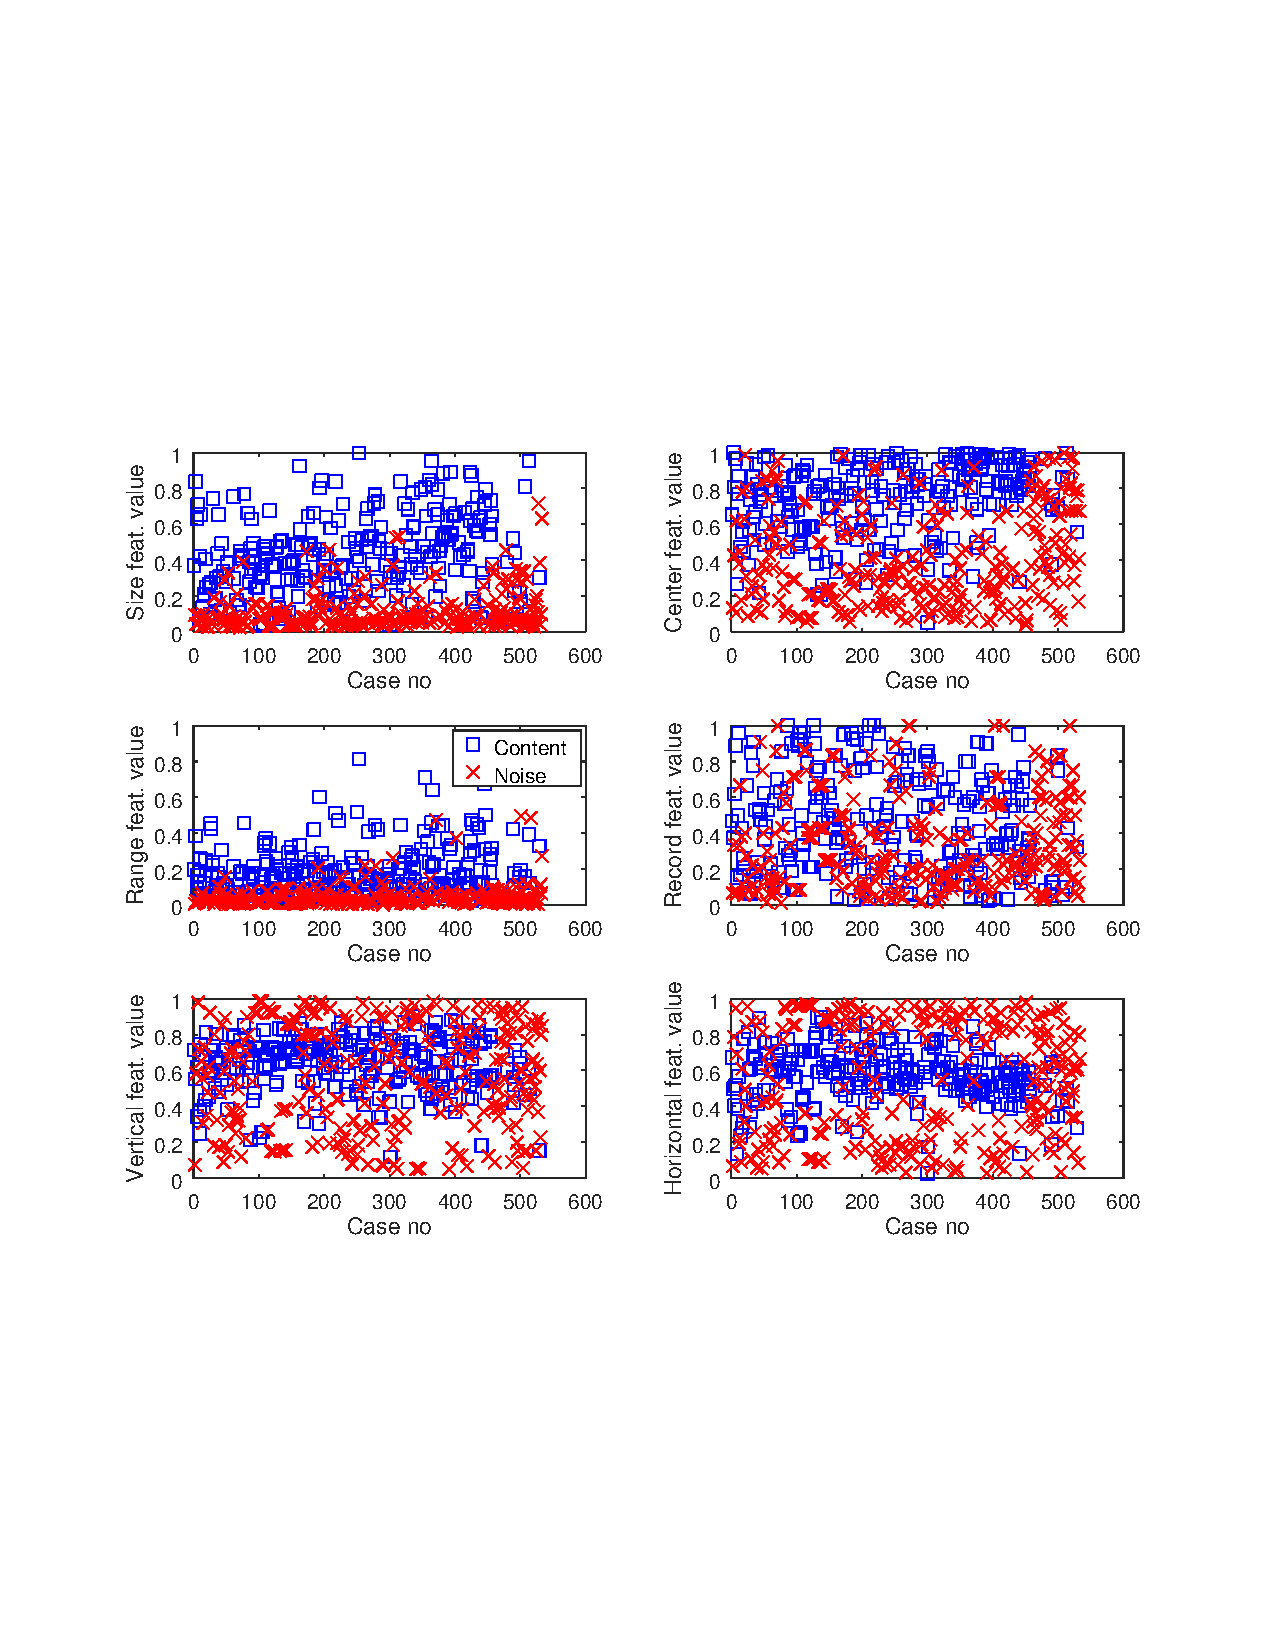
\includegraphics[trim={2.0cm 7.4cm 0.7cm 7.4cm}, clip,  width=\columnwidth]{img/dataset.pdf}
  \caption{Input dataset features: content vs noise. \textcolor{red}{esta figura fica boa quando imprime? Ser� que n�o seria melhor colocar s� 2 lado a lado? N�o esque�a de rotular direito as coordenadas - d� uma onferida em todas as tuas figuras antes de submeter e veja se est�o bem explicadas}}
  \label{fig:dataset}
\end{figure}

\section{Results}\label{sec:results}
We have used 5-fold cross-validation to evaluate the performance
of each model with respect to precision, recall, accuracy and F-Score. The
average results of 200 runs is shown in Tables \ref{tab:result} and
\ref{tab:resultnoise}.

When we omit the documents without structured content we get the results
shown in Table \ref{tab:result}. The best model was the Logistic Regressor (LR),
with 93.57\% F-score. In this application we should prioritize precision
(the web is vast and full of noise), with that in mind kNN performed a little
better, with almost 94\% precision. So, in a controlled enviromnment, where we
can guarantee the input will always contain structured content, the features we
elected were enough to achieve very good results with relatively simple models
(kNN and LR). No need to use more elaborate approaches and/or ensembles in this
setting.

\begin{table}[h]
\centering
\caption{Results using dataset containing only structured content documents.}
\label{tab:result}
\begin{tabular}{| l | l | l | l | l |}
\hline
Model & Precision & Recall & Accuracy & F-score \\ \hline
LR   & 93.30\% & \textbf{93.85}\% & \textbf{93.02}\% & \textbf{93.57}\% \\
GNB  & 91.97\% & 90.55\% & 90.62\% & 91.26\% \\
KNN  & \textbf{93.83}\% & 92.21\% & 92.59\% & 93.01\% \\
SVM  & 93.60\% & 92.20\% & 92.37\% & 92.90\% \\
EXT  & 91.88\% & 91.87\% & 91.23\% & 91.88\% \\
GB   & 90.75\% & 90.14\% & 89.74\% & 90.44\% \\
VOT  & 92.41\% & 92.20\% & 91.71\% & 92.31\% \\
STCK & 92.97\% & 92.20\% & 92.06\% & 92.59\% \\
\hline
\end{tabular}
\end{table}

When we consider the full dataset, including the documents without structured
content, we get the results shown in Table \ref{tab:resultnoise}. As expected
there is a drop in F-Score. The amount of unstructured documents corresponds,
roughly, to 18\% of the entire dataset and yet we were able attain negative
variations in F-Score lower than 1\%, for this reason we consider this results
to be very significant as they show it is possible to identify noise no matter
the content is structured or not. The most prominent drop, ironically, occurs
with Logistic Regressior (which performed best with only structured content
documents).
Gradient Boosting (GB), altough not the best performing model in either setting,
showed the lowest impact in F-Score. Another interesting result we see is that
all ensembles (VOT, STCK and GB) have relatively low drop in F-Score (the lowest
ones, in fact), with the exception of ExtraTrees (EXT) ensemble, which is the
second largest.
For this setting, where we have no guarantee that the documents have structured
content (only that they may have structured noise), the best option would be the
Voting heterogeneous ensemble with F-Score of 91.47\% and largest precision
(above 90\%).

\begin{table}[h]
\centering
\caption{Results using complete dataset (including unstructured documents).}
\label{tab:resultnoise}
\begin{tabular}{| l | l | l | l | l | l |}
\hline
Model & Precision & Recall & Accuracy & F-score & Drop \\ \hline
LR   & 87.97\% & 92.13\% & 89.45\% & 90.00\% & \textbf{\textcolor{red}{-3.57}}\% \\
GNB  & 89.69\% & 88.99\% & 89.47\% & 89.34\% & -1.92\% \\
KNN  & 89.72\% & 90.56\% & 90.02\% & 90.14\% & -2.87\% \\
SVM  & 89.51\% & 92.12\% & 90.77\% & 90.79\% & -2.11\% \\
EXT  & 88.80\% & 88.43\% & 88.71\% & 88.61\% & \textbf{\textcolor{red}{-3.27}}\% \\
GB   & 90.13\% & 88.97\% & 89.65\% & 89.55\% & \textbf{-0.89}\% \\
VOT  & \textbf{90.45}\% & \textbf{92.52}\% & \textbf{91.33}\% & \textbf{91.47}\% & -1.38\% \\
STCK & 89.93\% & 91.81\% & 90.73\% & 90.86\% & -1.73\% \\
\hline
\end{tabular}
\end{table}

In Table \ref{tab:resultcomp} we have compared our results with another,
state-of-the-art, approach found in the literature. We have compared the
performance of our classifiers in both settings (Logistic Regressor from Table
\ref{tab:result} and Voting Ensemble from Table \ref{tab:resultnoise}) with the
results published in \cite{TPC09}, using the same dataset (from
\cite{yamada2004testbed}).
The work in \cite{TPC09} deals specifically with
structured content, the authors have not measure its performance in the presence
of noise as we did in Table \ref{tab:resultnoise}.
We can see, in Table \ref{tab:resultcomp}, that our work outmatches the other
approaches (MDR by a large margin) even in the presence of unstructured content
documents.

\begin{table}[h]
\centering
\caption{Results comparison with other approaches.}
\label{tab:resultcomp}
\begin{tabular}{| l | l | l | l | l | l |}
\hline
Algorithm & Precision & Recall  & F-Score & Accuracy \\ \hline
TPC       & 90.40\%   & 93.10\% & 91.73\% & n/d \\
MDR       & 59.80\%   & 61.80\% & 60.78\% & n/d \\
 \hline \multicolumn{5}{|l|}{Our models} \\ \hline
LR & \textbf{95.45}\%   & 95.45\% & \textbf{95.45}\% & 94.80\% \\
VOT & \textbf{93.02}\%   & 90.91\% & \textbf{91.95}\% & 90.91\% \\
\hline
\end{tabular}
\end{table}

We show in Table \ref{tab:featsel} the best performing features for each model.
Almost all models used all features, this shows that all features are relevant
to the problem and somehow contribute to the solution. The exceptions are the
Logistic Regressor and SVM. The Logistic Regressor achieved the best results
without features ``center'' and ``vertical'' and SVM without feature ``center'',
that is probably due to the high correlation with other features. We can see in
Table \ref{tab:featcorr} thsat ``center'' has a considerable correlation with
``size'' and ``vertical'' with ``horizontal''.

\begin{table}[h]
\centering
\caption{Grid Search result: best set of features per algorithm.}
\label{tab:featsel}
\begin{tabular}{| l | l | l | l | l | l | l |}
\hline
Model     & Size   & Center & Range  & Record & Vertical & Horizontal \\ \hline
LR        & \cmark & \xmark & \cmark & \cmark & \xmark   & \cmark     \\
GNB       & \cmark & \cmark & \cmark & \cmark & \cmark   & \cmark     \\
EXT       & \cmark & \cmark & \cmark & \cmark & \cmark   & \cmark     \\
SVM       & \cmark & \xmark & \cmark & \cmark & \cmark   & \cmark     \\
kNN       & \cmark & \cmark & \cmark & \cmark & \cmark   & \cmark     \\
GB        & \cmark & \cmark & \cmark & \cmark & \cmark   & \cmark     \\
\hline
\end{tabular}
\end{table}

\begin{table}[h]
\centering
\caption{Grid Search result: algorithm parameters.}
\label{tab:params}
\begin{tabular}{| l | l |}
\hline
Model & Parameters \\ \hline 
LR        & $C=1.0$ \\ 
          & $penalty=L2$ \\
          & $warm\_start=True$ \\ \hline
GNB       & none \\ \hline
EXT       & $max\_features=0.8$ \\ 
          & $criterion=entropy$ \\
          & $warm\_start=False$ \\
          & $n\_estimators=31$ \\
          & $bootstrap=True$ \\
          & $min\_samples\_leaf=5$ \\ 
          & $min\_samples\_split=0.02$ \\ \hline
SVM       & $kernel=poly$ \\
          & $C=0.6$ \\
          & $gamma=0.188$ \\ 
          & $degree=3$ \\
          & $shrinking=True$ \\ \hline
kNN       & $weights=uniform$ \\
          & $p=3$ \\
          & $n\_neighbors=13$ \\ \hline
GB        & $min\_child\_weight=9 $ \\
          & $subsample=0.60$ \\ 
          & $n\_estimators=92$ \\ \hline
VOT       & $clfs=[GNB, SVM, kNN, GB]$ \\
          & $weights=[0.5, 1.0, 0.5, 0.5]$ \\ \hline
STCK      & $classifiers=[GNB, SVM, kNN, GB]$ \\
          & $meta\_classifier=LogisticRegression$ \\          
\hline
\end{tabular}
\end{table}

\section{Conclusion and Future Work}\label{sec:con}
In our research, thru observation, we have come up with the hypothesis depicted
here, for each feature and, thru experimentation, we have confirmed these
hypothesis in two different situations:
in a controlled setting (with 93.57\% F-Score using Logistic Regressor) and; in
an open environment (with 91.47\% F-Score using a heterogeneous voting
ensemble). We believe that these results are very good, specially
considering we are using only very basic information (size, position, etc.) to
distinguish between content and noise.

We have also demonstrated the relevance of these features to the problem
by testing every possible combination of features.

Nonetheless, there is always room for improvements. Adding other features
to the problem, perhaps using semantic features combined with the ones
proposed here, should be investigated. With an increased number of features,
testing all combinations becames prohibitive, other approaches should then be
employed (e.g., genetic algorithms) to find a good combination of features.


